% Created 2017-11-10 Fri 13:00
% Intended LaTeX compiler: pdflatex
\documentclass[11pt]{article}
\usepackage[utf8]{inputenc}
\usepackage[T1]{fontenc}
\usepackage{graphicx}
\usepackage{grffile}
\usepackage{longtable}
\usepackage{wrapfig}
\usepackage{rotating}
\usepackage[normalem]{ulem}
\usepackage{amsmath}
\usepackage{textcomp}
\usepackage{amssymb}
\usepackage{capt-of}
\usepackage{hyperref}
\usepackage{amsmath}
\author{Jake Brawer}
\date{\today}
\title{Assignment 7}
\hypersetup{
 pdfauthor={Jake Brawer},
 pdftitle={Assignment 7},
 pdfkeywords={},
 pdfsubject={},
 pdfcreator={Emacs 25.3.1 (Org mode 9.1.2)}, 
 pdflang={English}}
\begin{document}

\maketitle


\section*{1}
\label{sec:org16e6432}
Want to show that: $$ \pi(i)P(i,j) = \pi(j)P(j, i) \tag{1}$$ hold for Ehrenfest chains.
So we have:\\
$\pi(i) ~ Bin(n, \frac{1}{2}) \rightarrow {{n\choose i}}\frac{1}{2}^{n}$\\
$\pi(j) ~ Bin(n, \frac{1}{2})\rightarrow {{n\choose j}}\frac{1}{2}^{n}$

Thus the above simplifies to $$ {{n \choose i }}P(i, j) =  {{n \choose j }}P(j, i)$$
Given the nature of this particular chain  there are only two cases for $P$ that
we have to consider $P(i, i+1)$ and $P(i, i-1)$. Thus, in order to prove that
the chain is reducible it's sufficient to show that time-reversability holds in
these two cases.

\textbf{Case 1:} $P(i, j) = P(i, i+1)$\\

\begin{equation*}
   \pi(i)P(i, i + 1) = \pi(i + 1)P(i + 1, i)\\
   \rightarrow {{n \choose i}}P(i, i + 1) = {{n \choose j}}P(i +1, i)\\
\end{equation*}

So with $P(i + 1, i ) = \frac{i}{n} ,P(i , i + 1) = \frac{ n - i}{n}$\\
\begin{align*}
   & {{n \choose j }} \frac{ n - i}{n} = {{n \choose i}}\frac{i}{n}\\
   & \rightarrow \frac{n!}{i!(n-i-1)!}\frac{ n - i}{n} = \frac{n!}{(i+1)!(n - (i + 1))!} \frac{i}{n}\\
   & \rightarrow \frac{(n -1)!}{i!(n-i-1)!} = \frac{(n -1)!}{i!(n-i-1)!}
\end{align*}

\textbf{Case 2:} $P(i, j) = P(i, i - 1)$\\
\begin{equation*}
  & \pi(i)P(i, i -1) = \pi(i - 1)P(i -1 , i )\\
  & \rightarrow {{n \choose i}}P(i, i - 1) = {{n \choose j}}P(i  -1, i)\\
\end{equation*}
With  $ P(i , i -1 ) = \frac{i}{n} ,P(i - 1 , i ) = \frac{ n - (i - 1)}{n}\\$\\
\begin{align*}
  & {{n \choose i}} \frac{ i }{n} = {{n \choose j}}\frac{n - i}{n}\\
  & \rightarrow \frac{(n)!}{i!(n-i)!}\frac{i}{n} = \frac{n!}{(i - 1)!(n -
    (i - 1))!} \frac{n - (i - 1)}{n}\\
  & \rightarrow \frac{(n -1)!}{i!(n-i)!} = \frac{(n -1)!}{i!(n-i)!}
\end{align*}

And we're done!

\section*{2}
\label{sec:org24bd4a4}
\subsection*{a}
\label{sec:org8c0d4e7}
\begin{verbatim}

MC <- function(reps, scale, f, m ,sd){
  path <- numeric(reps)
  initial <- 3
  state <- initial
  path[1] <- initial
  for(i in 2:reps)
  {
    candidate <- runif(1,state - scale,state + scale)
    ratio <- f(candidate, m , sd)/f(state, m, sd)

    if(runif(1) < ratio) state <- candidate

    path[i] <- state
  }
  return(path)
}


\end{verbatim}

\subsection*{b}
\label{sec:org796274a}

\begin{verbatim}
f1 <- function(x, m, sd){
  return(dnorm(x, mean=m, sd=sd))
}
f1(0, 0, .1)

plot(MC(100000, 1, f1, 3, 0.001))
\end{verbatim}

\begin{center}
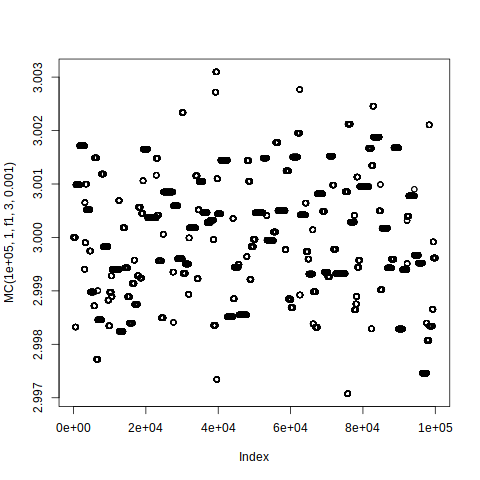
\includegraphics[width=.9\linewidth]{fig0.png}
\end{center}

\begin{verbatim}
library(MASS)  # for truehist function
truehist(MC(100000, 1, f1, 3, 0.001))

\end{verbatim}

\begin{center}
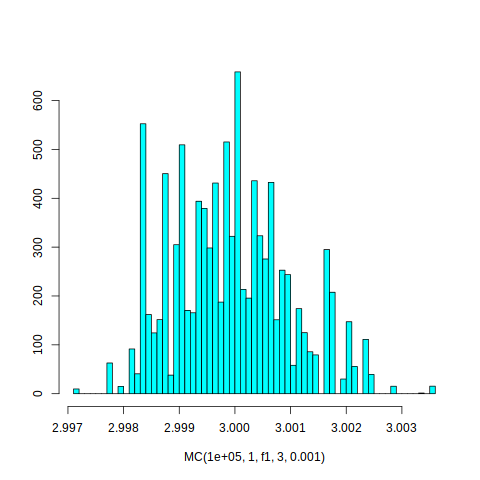
\includegraphics[width=.9\linewidth]{hist.png}
\end{center}


These graphs looks sparse and very spread out, but this is likely due to the large scale value relative to our standard deviation. That is we are walking around the distribution by step size of 1 yet, the majority of the density is contained within +- 0.001 of the mean.

\subsection*{c}
\label{sec:org2784d84}
\begin{verbatim}
plot(MC(100000, 0.001, f1, 3, 0.001))

\end{verbatim}

\begin{center}
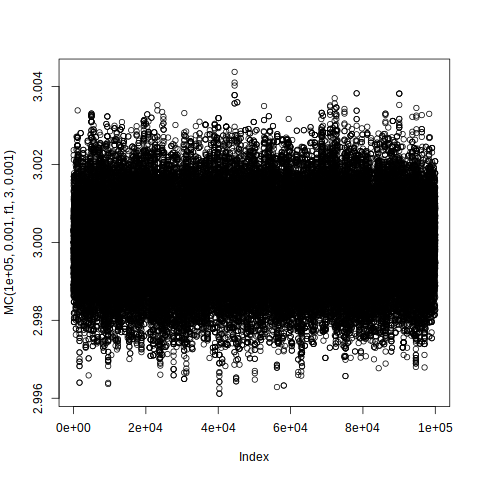
\includegraphics[width=.9\linewidth]{figy.png}
\end{center}

\begin{verbatim}
truehist(MC(100000, 0.001, f1, 3, 0.001))

\end{verbatim}

\begin{center}
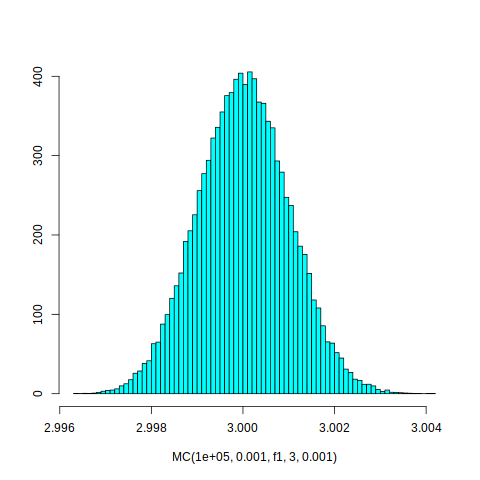
\includegraphics[width=.9\linewidth]{hist2.png}
\end{center}


These graphs look more normal likely due to the fact that scale value is in line with the SD.

\subsection*{d}
\label{sec:org653339d}

\begin{verbatim}
plot(MC(100000, 0.001, f1, 0, 1))

\end{verbatim}

\begin{center}
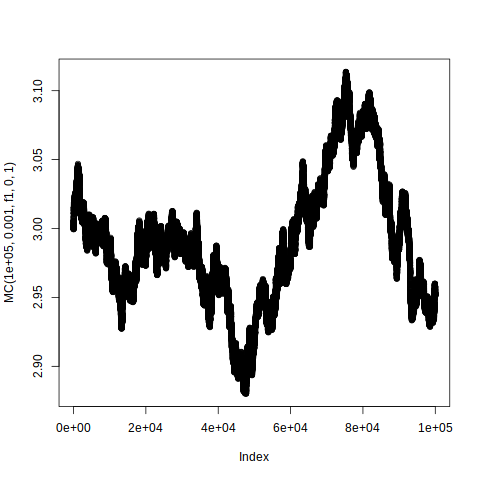
\includegraphics[width=.9\linewidth]{figy2.png}
\end{center}

\begin{verbatim}
truehist(MC(100000, 0.001, f1, 0, 1))

\end{verbatim}

\begin{center}
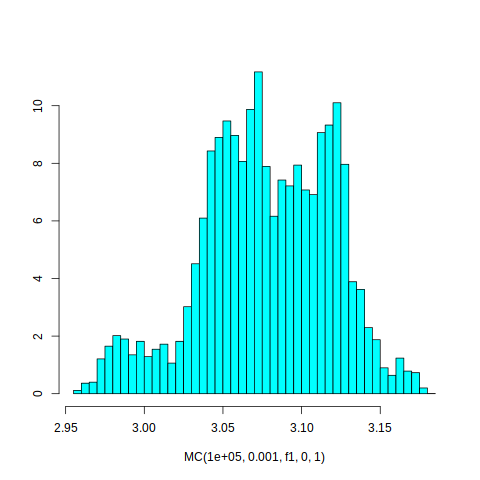
\includegraphics[width=.9\linewidth]{hist3.png}
\end{center}

These graphs look weird. Our initial starting position is very far away from the mean, and our step size is very small which means we are not getting good samples.

\section*{3}
\label{sec:org7f878b5}
\subsection*{a}
\label{sec:orgfd8e86b}
$Q = $
\begin{bmatrix}
  0 & \frac{1}{3} & \frac{1}{3} & \frac{1}{3} & 0\\
  \frac{1}{3} & 0 & \frac{1}{3} & \frac{1}{3} & 0 \\
  \frac{1}{3} & \frac{1}{3} & 0 & \frac{1}{3} & 0\\
  \frac{1}{4} & \frac{1}{4} & \frac{1}{4} & 0 &\frac{1}{4}\\
  0 & 0 & 0 & 1& 0 
\end{bmatrix}

$\pi = \[ \frac{3}{14}, \frac{3}{14}, \frac{3}{14}, \frac{4}{14}, \frac{1}{14}\]$

\subsection*{b}
\label{sec:org4a79366}
Given that modifying Q requires application of an algorithm, I implemented the algorithm in R!.
\begin{verbatim}

mh <- function(Q, p){
  P <- matrix(rep(0, 25), byrow=TRUE, ncol=5)

  row <- dim(P)[1]
  col <- dim(P)[2]

  for(i in 1:row)
  {
    for(j in 1:col)
    {
      h <- p[j] * Q[j, i]
      g <- p[i] * Q[i, j]
      # Don't want to divide by 0
      hg <- if (is.nan(h/g))  1 else min(1, h/g)

      if(i != j)
      {
        P[i, j]  = Q[i, j] * hg
      }
    }
  }

  # Handle the diagonal entries
  for(k in 1:row)
  {
    P[k, k] = 1 - sum(P[k, ])
  }

  return(P)
}

Q <- matrix(c(0, 1/3, 1/3, 1/3, 0,
              1/3, 0, 1/3, 1/3, 0,
              1/3, 1/3, 0, 1/3, 0,
              1/4, 1/4, 1/4, 0, 1/4,
              0, 0, 0, 1, 0), byrow=TRUE, ncol=5)

stat <- c(1/15, 2/15, 3/15, 4/15, 5/15)

P <- mh(Q, p )
P
\end{verbatim}

\subsection*{c}
\label{sec:org77c313b}
\begin{verbatim}
stat
\end{verbatim}

\begin{center}
\begin{tabular}{r}
0.0666666666666667\\
0.133333333333333\\
0.2\\
0.266666666666667\\
0.333333333333333\\
\end{tabular}
\end{center}

\begin{verbatim}
stat %*% P
\end{verbatim}

\begin{center}
\begin{tabular}{rrrrr}
0.0666666666666667 & 0.133333333333333 & 0.2 & 0.266666666666667 & 0.333333333333333\\
\end{tabular}
\end{center}

\subsection*{d}
\label{sec:org7349f48}
\begin{verbatim}
simPath <- function(size, P ){
# Randomly chose  a start position
  start <- c(0, 1, 0, 0 ,0, 0)
  stateHist <- rep(0, size) # Stores counts for state visitation
  prev <- start
  for(i in 1:size)
  {
    prev <- sample(1:5, size = 1, prob = P[prev, ])
    stateHist[i] <- prev
  }

  return(stateHist)
}

reps <- 100000
table(simPath(reps, P))
\end{verbatim}

\begin{center}
\begin{tabular}{rr}
1 & 6806\\
2 & 13249\\
3 & 19972\\
4 & 26563\\
5 & 33410\\
\end{tabular}
\end{center}

If we normalize the table we get:

\begin{verbatim}
table(simPath(reps, P) ) / reps
\end{verbatim}

\begin{center}
\begin{tabular}{rr}
1 & 0.06712\\
2 & 0.13284\\
3 & 0.19906\\
4 & 0.26907\\
5 & 0.33191\\
\end{tabular}
\end{center}


Observe the similarity to the standing dist. derived above:

\begin{verbatim}
stat
\end{verbatim}

\begin{center}
\begin{tabular}{r}
0.0666666666666667\\
0.133333333333333\\
0.2\\
0.266666666666667\\
0.333333333333333\\
\end{tabular}
\end{center}

\section*{4}
\label{sec:org7d3ef8a}
\subsection*{a}
\label{sec:org9da819e}

The acceptance probability in the original M-H algorithm looks like:\\
$$A(x,y) = min\left\{ 1, \frac{\pi(y)Q(y, x)}{\pi(x)Q(x,y)}\right\}$$
From the problem we are given that $ Q(x, y) = g(y)$ so:\\
$$A(x,y) = min\left\{ 1, \frac{\pi(y)g(x)}{\pi(x)g(y)}\right\}$$
$\pi$ by definition is a pdf (pr pmf) so $\pi = f$ and\\
$$A(x,y) = min\left\{ 1, \frac{f(y)g(x)}{f(x)g(y)}\right\}$$
and we are done.

\subsection*{b}
\label{sec:orgb83fd77}

Here's how the function looks:
\begin{verbatim}
f <- function(x){
  return(sqrt(1.7 + sin(2.5 * x))* exp(-((abs(x)^1.5) / 3)))
}

plot(f, -10, 10)
\end{verbatim}

\begin{center}
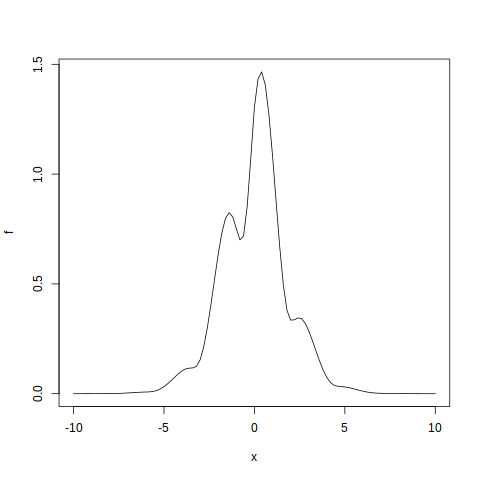
\includegraphics[width=.9\linewidth]{fig1.png}
\end{center}


\begin{verbatim}
MCMC <- function(size){
  path <- numeric(size)
  initial <- rcauchy(1)
  state <- initial
  path[1] <- initial
  for(i in 2:size)
  {
    candidate <- rcauchy(1)
    ratio <- f(candidate)/f(state)

    if(runif(1) < ratio) state <- candidate

    path[i] <- state
  }
  return(path)
}

truehist(MCMC(10000))
con <- integrate(f, -Inf, Inf)$value
f1 <- function(x){f(x)/con}
plot(f1, -10, 10, add=T, lwd=2, col=2)
\end{verbatim}

\begin{center}
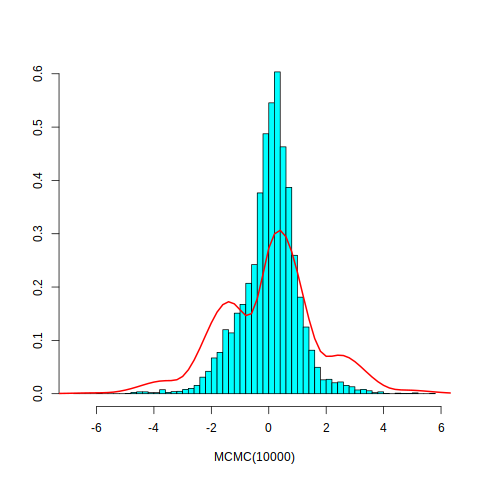
\includegraphics[width=.9\linewidth]{fig2.png}
\end{center}
\subsection*{c}
\label{sec:orgb0e2790}

\begin{verbatim}
reps <- 10000
samp <- MCMC(reps)

n <- samp[samp < 2.38]
length(n)/reps


\end{verbatim}

\begin{verbatim}
0.9852
\end{verbatim}
\end{document}